
%\subsubsection{Introduction}
%\label{intro}

In this work we are interested in the measurement of the Standard Model (SM) Triple Gauge Couplings (TGCs). This is a classic test of the SM and a possible measurement of deviations from its expectations would signify an invaluable piece of information for the theory beyond the SM. A consistent way to parametrize such possible deviations is through the SM Effective Field Theory (EFT) approach.
We are going to consider the SM EFT as defined in \cite{Azatov:2017kzw,Azatov:2019xxn}, in particular we are going to focus on the measurement of the EFT operator $\mathcal{O}_{3W}$, see Table~\ref{tab:dim6ops}, which is associated to the the anomalous triple gauge coupling (aTGC) $\lambda_z$.





A precise determination of the TGC stems from the measurement of  the $2\to 2$  cross section $\sigma ( q\bar q \rightarrow VV )$~\cite{Sirunyan:2017bey,Aad:2016ett}. Naive dimensional analysis and standard EFT reasoning predicts that the energy scaling of such cross-section is given by
\bea
\label{eq:sigtt}
\begin{split}
\sigma(q\bar q \to V V)\sim \frac{g_{\text{SM}}^4}{E^2}\bigg[ 
 1 & +\overbrace{c_i\frac{E^2}{\Lambda^2}}^\text{BSM$_6\times\,$SM}
       +\overbrace{c_i^2 \frac{E^4}{\Lambda^4}}^\text{BSM$_6$$^2$}+ \dots \bigg]\, , 
\end{split} \label{genxsec}
\eea
where the first factor $g_\text{SM}^4/E^2$ accounts for the energy flux of the initial quarks, $c_i$ are the  relevant Wilson coefficients, and we have omitted numerical factors.
In (\ref{genxsec}) we have explicitly indicated dimension six squared  ($\text{BSM$_6$$^2$}$) and SM-dimension six interference terms ($\text{BSM$_6\times\,$SM}$).\footnote{Note that operators of dimension 7 necessarily violate either baryon or lepton number. We assume the scale of such symmetry violation to be very large and therefore irrelevant for diboson physics at the LHC.}  The ellipses in (\ref{genxsec}) are due to corrections from operators of dimension $\geq 8$, which we will neglect. The leading  such term is an interference term of the type $\text{BSM$_8\times\,$SM}$ and it is of order $O(E^4/\Lambda^4)$.

A closer inspection however reveals that the  $2\to 2$ diboson production through the dimension six operator $\mathcal{O}_{3W}$  has an interference piece with a suppressed energy scaling. 
Indeed, the energy scaling of such process is  
\begin{equation}
\sigma ( q\bar q \rightarrow VV ) \sim \frac{g_\text{SM}^4}{E^2}\bigg[  1 +  C_{3W}\frac{m_V^2}{\Lambda^2}  +C_{3W}^2 \frac{E^4}{\Lambda^4}  + O(E^4/\Lambda^4) \bigg]. \label{sup}
\end{equation} 
This is a consequence of the  helicity selection rules, see    
\cite{Dixon:1993xd,Azatov:2016sqh,Azatov:2017kzw,Panico:2017frx}.
The suppressed energy scaling can be problematic for the correct EFT  
interpretation of the $\sigma(q\bar q \to V V)$ measurement. 
Namely, in view of (\ref{sup}), the sensitivity on $C_{3W}$ is largely 
dominated by the quadratic piece $\text{BSM}_6^2$, which is 
$O(E^4/\Lambda^4)$. 
 Furthermore, in this case, the measurements become insensitive to the sign of the Wilson coefficient.
The main objective of the present work is to 
improve the sensitivity to the linear piece $\text{BSM$_6\times\,$SM}$.
We will present two classes of solutions to achieve this goal. Firstly, in section \ref{angs} we  will show that the differential angular cross-section 
 of the process $q\bar q \rightarrow VV\rightarrow 4\psi$ has a large sensitivity on $\text{BSM$_6\times\,$SM}$ compared to the inclusive cross-section.   Secondly, in section \ref{jetsol} we will show that accounting for extra radiation $q\bar q \rightarrow VV+j$ also results in an improved sensitivity on the leading piece $\text{BSM$_6\times\,$SM}$.
These measurements are specially interesting in a HL/HE phase of the LHC, for which we show the prospects below.% in  section~\ref{res}.

%\subsubsection{Solutions}


\begin{figure}[t]
\begin{center}
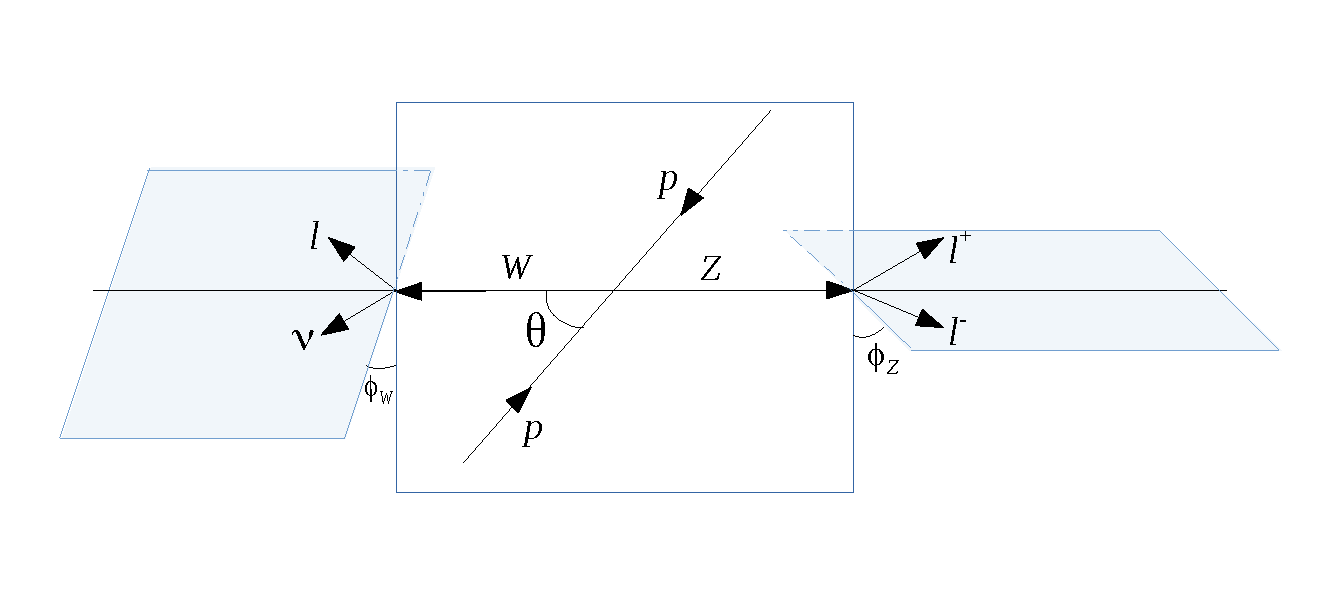
\includegraphics[scale=0.4]{\main/section4/plots/angles}
\end{center}
\vspace{-.3cm}
\caption{Angles for $2\to 4$ scattering. \label{fig:ang}}
\end{figure}

Next we will present two ways to  improve the sensitivity to the aTGC $\lambda_z$ by restoring the energy growth
$g_\text{SM}^4/E^2\left[1+c_i E^2/\Lambda^2+  \dots\right]$ of the interference piece $\text{BSM$_6\times\,$SM}$ of the  $\mathcal{O}_{3W}$ operator.\\

\noindent
{\bf Interference resurrection via angular distributions}\\
\label{angs}
The first way of enhancing the interference term is by noting that in a collider experiment instead of the  $2\to 2$ process we actually measure a $2\to 4$ scattering, i.e. vector bosons decay into fermions $q\bar q\to V_1V_2\to 4 \psi$.  
%
Let us start by considering  the differential cross section for the production of the polarized particles $W_{T+} Z_T \rightarrow W_{T+}  l_+ \bar l_-$\footnote{ We ignore the  longitudinal Z polarization which is subdominant at the LHC \cite{Baur:1994ia}.}
\be
\frac{d\sigma(q\bar q \rightarrow W_{T_+} l_- \bar l_+)}{d\text{LIPS} } =
 \frac{1}{2 s}  \frac{ \left|\sum_i  
(  {\cal M}^\text{SM}_{q\bar q \rightarrow W_{T_+}Z_{i}}+
 {\cal M}^\text{BSM}_{q\bar q \rightarrow W_{T_+}Z_{i}}
)
  {\cal M}_{Z_{i}\to  l_- \bar l_+}   \right|^2}{(k_Z^2-m_Z^2)^2+m_Z^2\Gamma_Z^2} 
\,  , \label{xsecan}
\ee
where   sum runs over intermediate Z polarizations and $d\text{LIPS}\equiv (2\pi)^4\delta^4(\sum p_i -p_f) \prod_i {d^3 p_i}/\left(2 E_i(2\pi)^3\right)$ is the Lorentz Invariant differential 
Phase Space.  
%
Then in the narrow width approximation the leading contribution to the interference, i.e. the cross term $\text{SM}\times\text{BSM}_6$ in \ref{xsecan},   is given by
$
d\sigma_\text{int}(q\bar q \rightarrow W_{T_+} l_- \bar l_+)/ d\phi_Z \propto E^2/\Lambda^2 \cos(2\phi_Z) 
$, 
where  $\phi_Z$  is the azimuthal angle between the plane defined by the decaying leptons and the plane defined by the collision and WZ momenta, see Fig.~\ref{fig:ang}.  Note that $d\sigma_\text{int}(q\bar q \rightarrow W_{T_+} l_- \bar l_+)/ d\phi_Z $ has the energy growth expected from naive dimensional analysis, see  Eq.~\ref{genxsec}.
An analogous derivation goes through if we also consider the decay of the W gauge boson. The differential interference term   for the process $q\bar q\to WZ\to 4 \psi$ is  unsuppressed and modulated as
\bea
 \frac{d\sigma_\text{int}(q\bar q \rightarrow W Z\rightarrow  4\psi)}{d\phi_Z\, d\phi_W}  \propto \frac{E^2}{\Lambda^2}\left( \cos(2\phi_Z)+\cos(2\phi_W)\right) , \label{simp}
\eea
where $\phi_{W,Z}$ are the corresponding azimuthal angles. 
Integrating  \ref{simp} over the fermion phase space the   interference term vanishes as expected from the discussion above. 
Since the dependence on the two azimuthal angles is additive, integrating  over $\phi_W$ leads to a differential cross-section that is modulated by $\cos(2\phi_Z)$ and that features $E^2/\Lambda^2$ energy growth. 
We will use the result in Eq.~\ref{simp}  to prove the aTGC $\lambda_Z$, with an increased  overall sensitivity  to both the magnitude and sign of the Wilson coefficient.


 
%\subsubsection*{Angle ambiguities} 
 Following Ref.~\cite{Panico:2017frx}, we make a few remarks on the experimental measurement  of $\phi_{Z,W}$ in Eq.~\ref{simp}.
 The angle $\phi_Z$  can be determined up to an ambiguity  $\phi_Z\leftrightarrow \phi_Z \pm \pi$,
 since experimentally we can only measure the charges but not the helicities of the  leptons from $Z$  decay.
 The reconstruction of the $W$  azimuthal  angle $\phi_W$ in the $l\nu$ final state  suffers from an ambiguity  $\phi_W \leftrightarrow \pi-\phi_W$ due to the twofold ambiguity in the determination of the neutrino momentum.
Interestingly, none of these ambiguities  affects  Eq.~\ref{simp}.\\

\noindent
{\bf Interference resurrection via jet emission}\\
\label{jetsol}
A second way to resurrect the expected energy growth of the 
interference term is based on the observation that the helicity 
selection rule holds only at leading-order \cite{Azatov:2017kzw}. 
So the next-to-leading-order (NLO) effects will necessarily lead to the 
enhancement of the interference.
Virtual effects are expected to be suppressed by a factor ${\cal{O}}( 
\alpha_s/4\pi)$ with respect to the contributions coming from azimuthal modulation discussed in the previous section. A complete study at NLO accuracy for the operator ${\cal O}_{3W}$ together with its CP-odd counterpart can be found in~\cite{Azatov:2019xxn}.
Alternatively we will consider processes with an extra hard jet emission, which will improve on the  signal over the  background ratio. 
 In this case,  since   we are dealing with the hard
  $2\to 3$ process,
 the same polarization configuration $q\bar{q}\to V_{\pm}V_{\pm}g_{\mp}$ is allowed both in SM and in the BSM five point amplitude with the $\mathcal{O}_{3W}$ insertion. Therefore the interference is not suppressed and the leading quadratic energy scaling is restored by requiring an extra (hard) QCD radiation.\\

\noindent
{\bf Results}\\
\emph{HL-LHC.} In order to test the sensitivity of the High-Luminosity (HL) phase of the LHC on the $\mathcal{O}_{3W}$ with the proposed solution to the non-interference behaviour we proceed in the following way. We generate with {\tt MadGraph5 aMC@NLO}~\cite{Alwall:2014hca} parton level events for $pp \to W^{\pm} Z $ decaying into a four leptons (electron and muon) final state together with events for the same process where we allow for a jet emission in the initial state. We perform two different analyses (see~\cite{Azatov:2017kzw} for more details): an inclusive one where we restrict to events up to $p_T^j<100\;$ GeV and do not bin on the $\phi_Z$ variable and an exclusive one where we bin both on the jet transverse momentum and on $\phi_Z$, where for the latter we define two bins with the threshold $|\cos(\phi_Z)|=1/\sqrt{2}$. All together the results for the bound on the $C_{3W}$ Wilson coefficient are reported in Fig.~\ref{fig:LHC13} as a function of the maximum transverse mass of the $WZ$ system, which allows to have an estimate of the validity of the EFT computation, see again~\cite{Azatov:2017kzw} for a detailed discussion~\footnote{These results are obtained by keeping both the linear and the quadratic terms in the cross section determination.}.

One might wonder if a simulation beyond the parton level accuracy might spoil these results. To this end we have performed a more detailed simulation by showering the events through {\tt PYTHIA 8}~\cite{Alwall:2014hca} and simulating the detector response via {\tt Delphes 3}~\cite{deFavereau:2013fsa}. By analysing the density of events in the two azimuthal bins we found that with respect to the parton level case the relative difference is of at most a few \%, thus making our parton level analysis solid.


  
  \begin{figure}[ht]
\begin{center}
 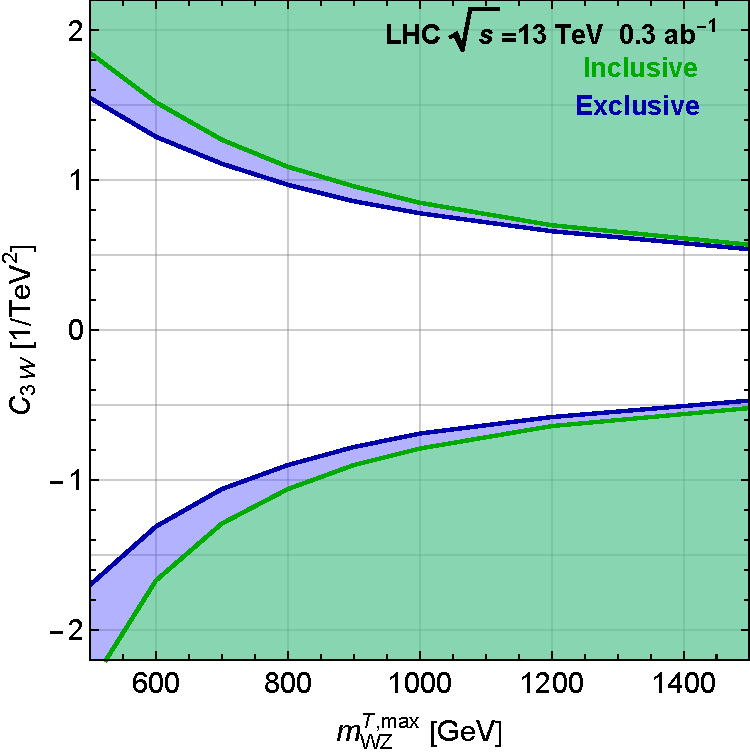
\includegraphics[width=0.39\textwidth]{\main/section4/plots/LHC13_300.pdf}{}\hspace{2cm}
 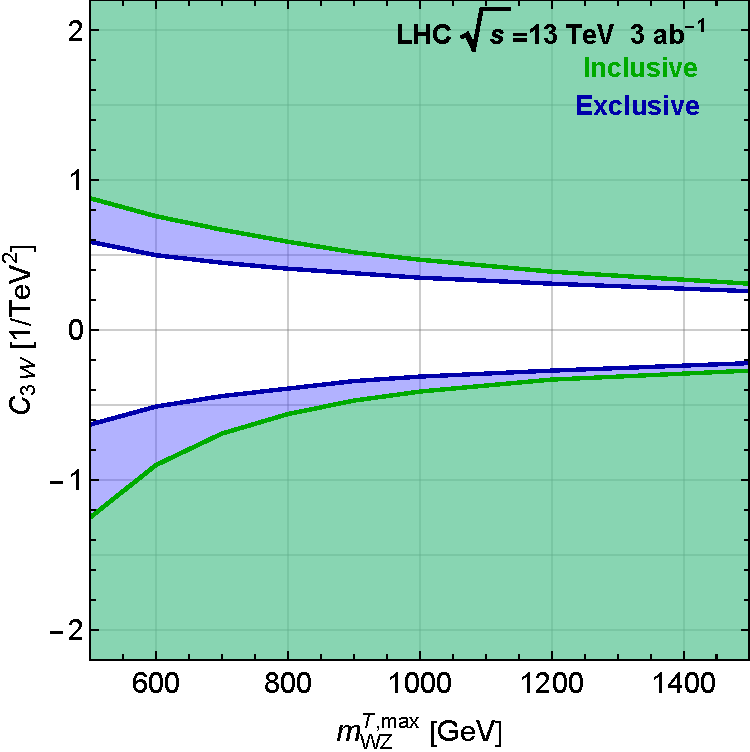
\includegraphics[width=0.39\textwidth]{\main/section4/plots/LHC13_3000.pdf}{}
\end{center}
\caption{Bounds on the $C_{3W}$ Wilson coefficient for the inclusive and exclusive categories at the LHC 13 for 300 fb$^{-1}$ (left) and 3000 fb$^{-1}$ (right) of integrated luminosity.}
\label{fig:LHC13}
\end{figure}


\noindent
\emph{HE-LHC.}
We now estimate the reach of a future HE phase of the LHC with
$\sqrt{s}=27\;$TeV. For these preliminary results we adopt the same binning, both in $\phi_Z$ and in jet transverse momentum, of the previous section. We show the results in Fig.~\ref{fig:LHC27}. We found a slight increase of order $~30\%$ on the reach on $C_{3W}$. We expect that a dedicated HE analysis will lead to a further improvement of these bounds; this can be done by exploiting in a more efficient way the high energy tails of the differential distributions. In~\cite{Azatov:2019xxn} we also present a complete NLO study for the HE-LHC stage. 


  \begin{figure}[ht]
\begin{center}
 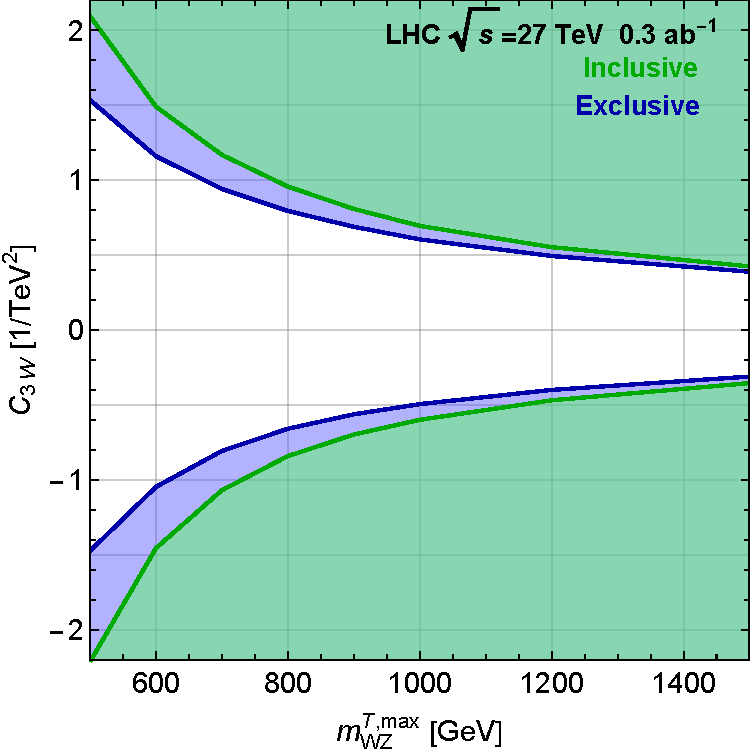
\includegraphics[width=0.39\textwidth]{\main/section4/plots/LHC27_300.pdf}{}\hspace{2cm}
 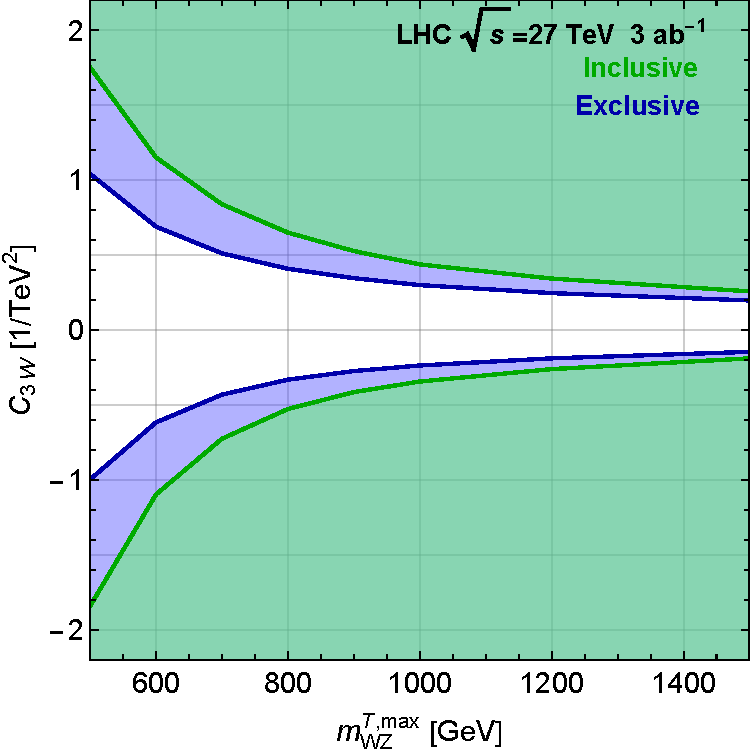
\includegraphics[width=0.39\textwidth]{\main/section4/plots/LHC27_3000.pdf}{}
\end{center}
\caption{Bounds on the $C_{3W}$ Wilson coefficient for the inclusive and exclusive categories at the LHC 27 for 300 fb$^{-1}$ (left) and 3000 fb$^{-1}$ (right) of integrated luminosity.}
\label{fig:LHC27}
\end{figure}


